\section{Theory of Relations}

  The most intuitive way to store data is with a \textit{table}, which is called a relational data model, which is the norm since the 1990s. We will first talk about the structure, then the operations, and finally some constraints. 

\subsection{Structure}

  \begin{definition}[Relation]
    A \textbf{relation} is a set or multiset $R$ with the following data structure. 
    \begin{enumerate}
      \item Each element $r \in R$ is called a \textbf{tuple}/\textbf{row}, with the form $r = (a_1 \in T_1, \ldots, a_n \in T_n)$. Despite its name and our use of indices, the tuple itself is \textit{not ordered}. 
      \item Each $T_i$ is a primitive\footnote{loosely defined here} type (e.g. int float, string, but not a list or set).\footnote{Note that this is also a form of constraint on our data, but the types are usually defined under structure.}
      \item Each $T_i$ is given an alphanumeric name $A_i$ as a variable, called the \textbf{attribute}. We denote $\mathbf{A}$ as the set of the attribute of relation $R$. 
      \item The \textbf{schema} of $R$ tells us a summary of its structure: $R(A_1 \; T_1, A_2 \; T_2, \ldots, A_n \; T_n)$. 
      \item Given a time parameter $t$, $R_t$ represents the \textbf{instance} of the relation $R$ at time $t$. 
    \end{enumerate}
    Given these names, we can visualize relations as tables, tuples as rows, and attributes as columns. 
  \end{definition} 

  We introduce this in this abstract way because there are many implementation differences between DBMSs. For example, the set of available primitive types may differ, or we may be able to define attribute names with special characters. Even in \textit{temporal databases}, we may also keep track of the history of its instances rather than just the current instance. 

  \begin{example}[Schemas]
    Here are a few schemas, which has the name of the relation followed by the attributes and its types. 
    \begin{lstlisting}
      Beer (name string, brewer string)
      Serves (bar string, price float)
    \end{lstlisting}
    Note that this is analogous to a function declaration in C++. 
  \end{example}  

  \begin{definition}[Compatiblity]
    Two relations $R$ and $S$ are \textbf{compatible}, denoted $R \simeq S$, if they have the same schema (same set of attribute types and names). 
  \end{definition}

  While we have not talked about any types yet, there is a common one that we should mention now. 

  \begin{definition}[Null]
    A \textbf{null} value, denoted with $\omega$ indicates an unknown but not empty value. The specific behavior of this value will be covered when we get into SQL implementations. 
  \end{definition}

\subsection{Operations and Relational Algebra}

    We have just defined sets, and the natural thing to do is to construct functions on sets, i.e. what operations are legal. We introduce this with \textit{relational algebra}, which gives a powerful way to construct new relations from given relations. Simply put, an algebra is an algebraic structure with a set of operands (elements) and operators.\footnote{Not the technical definition.}

    \begin{definition}[Relational Algebra] 
      A \textbf{relational algebra} consists of a set of operations $O$ grouped into 4 broad categories. 
      \begin{enumerate}
        \item \textit{Set Operations}. Union, intersection, and difference. 
        \item \textit{Removing}. Selection removes tuples and projection removes attributes. 
        \item \textit{Combining}. Cartesian products, join operations. 
        \item \textit{Renaming}. Doesn't affect the tuples, but changes the name of the attributes or the relation itself. 
      \end{enumerate}
    \end{definition}

    Let's take a look at each of these operations more carefully, using the following relation. 

    \begin{figure}[H]
      \centering
      \begin{tabular}{|l|l|r|}
      \hline
      \rowcolor[HTML]{E26B0A} 
      \textcolor{white}{\textbf{bar}} & \textcolor{white}{\textbf{beer}} & \textcolor{white}{\textbf{price}} \\ \hline
      \rowcolor[HTML]{FBCEB1}
      The Edge & Budweiser & 2.50 \\ \hline
      \rowcolor[HTML]{FBCEB1}
      The Edge & Corona & 3.00 \\ \hline
      \rowcolor[HTML]{FBCEB1}
      Satisfaction & Budweiser & 2.25 \\ \hline
      \end{tabular}
      \caption{The example relation, which we will denote \texttt{serves}, which we will use to demonstrate the following operations.} 
      \label{fig:serves}
    \end{figure} 

  \subsubsection{Set Operations}

    \begin{definition}[Union]
      Given $R \simeq S$, $R \cup S$ is the set/multiset of tuples in either $R$ or $S$. 
    \end{definition}

    \begin{definition}[Intersection]
      Given $R \simeq S$, $R \cap S$ is the set/multiset of tuples in both $R$ or $S$. 
    \end{definition}

    \begin{definition}[Difference]
      Given $R \simeq S$, $R - S$ is the set of tuples in $R$ but not $S$, or the multiset that keeps track of counts in $R$ and $S$. 
    \end{definition}

    Note that this set is not minimal. 

    \begin{lemma} 
      Given $R \simeq S$, 
      \begin{align}
        R \cap S  & = R - (R - S) \\ 
                  & = S - (S - R) \\ 
                  & = R \bowtie S
      \end{align}
    \end{lemma}
    \begin{proof}
      The natural join will check for all attributes in each schema, but sine we assumed that they had the same schema, it must check for equality over all attributes.
    \end{proof}

    \begin{example}[Symmetric Difference of Relations]
      Let $R(A,B,C) = \{(1,2,3), (4,2,3), (4,5,6), (2,5,3), (1,2,6)\}$ and\\
      $S(A,B,C) = \{(2,5,3), (2,5,4), (4,5,6), (1,2,3)\}$\\
      Compute $(R - S) \cup (S - R)$ (symmetric difference). Identify one tuple in the result.

      \begin{enumerate}
        \item $(4,5,6)$ This tuple appears in both R and S, so it's not in the symmetric difference.
        
        \item $(2,5,3)$ This tuple appears in both R and S, so it's not in the symmetric difference.
        
        \item $\mathbf{(1,2,6)}$ This tuple appears only in R, so it's in R - S and thus in the symmetric difference.
        
        \item $(1,2,3)$ This tuple appears in both R and S, so it's not in the symmetric difference.
      \end{enumerate}
    \end{example}

  \subsubsection{Projection and Selection}

    \begin{definition}[Selection]
      The \textbf{selection} operator $\sigma_p$ filters the tuples of a relation $R$ by some condition $p$. 
      \begin{equation}
        \sigma_p (R)
      \end{equation}
      It must be the case that $p$ is deducible by looking only at that row, but it may not be (e.g. the condition where the count of an attribute in the row passes a threshold). 
    \end{definition}

    \begin{definition}[Projection]
      Given that $L \subset \mathbf{A}$ is a a subset of $R$'s attributes, the \textbf{projection} operator $\pi_L$ filters the attributes of a relation $R$. 
      \begin{equation}
        \pi_L (R)
      \end{equation}
    \end{definition}

    \begin{example}[Projection Operation]
      Given $R(A,B,C) = \{(1,2,3), (4,2,3), (4,5,6), (2,5,3), (1,2,6)\}$\\
      Compute $\pi_{C,B}(R)$ and identify one tuple.

      \begin{enumerate}
        \item $(4,2)$ 
        \item $\mathbf{(3,2)}$ This is correct. 
        \item $(4,2,3)$ Projection onto C,B should only have two attributes, not three.
        \item $(2,3)$ This reverses the specified projection order of C,B.
      \end{enumerate}
    \end{example}

  \subsubsection{Product and Join}

    \begin{definition}[Cartesian Product]
      The \textbf{cartesian product} of two not-necessarily compatible relations $R$ and $S$ is the relation 
      \begin{equation}
        R \times S = \{r \in S, s \in S\} 
      \end{equation}
      which has a length of $|R| \times |S|$. It is commutative (again, tuples are not ordered despite its name), and if $S$ and $R$ have the same attribute name $n$, then we usually prefix it by the relation to distinguish it: $S.n, R.n$. 
    \end{definition}

    \begin{definition}[Theta-Join]
      The \textbf{theta-join} with \textbf{join condition/predicate} $p$ gives 
      \begin{equation}
        R \bowtie_p S = \sigma_p (R \times S)
      \end{equation}
      If $p$ consists of only equality conditions, then it is called an \textbf{equi-join}. 
    \end{definition}

    \begin{example}[Conditional Join Query]
      Given $R(A,B) = \{(1,2), (3,4), (5,6)\}$ and\\
      $S(B,C,D) = \{(2,4,6), (4,6,8), (4,7,9)\}$\\
      Compute the join with conditions $R.A < S.C$ AND $R.B < S.D$.

      \begin{lstlisting}[basicstyle=\ttfamily]
        SELECT A, R.B, S.B, C, D
        FROM R, S
        WHERE R.A < S.C AND R.B < S.D
      \end{lstlisting}

      \begin{enumerate}
        \item $(5,6,2,4,6)$ This doesn't satisfy R.A < S.C as 5 > 4.
        
        \item $(1,2,4,4,6)$ The values don't properly satisfy both conditions.
        
        \item $(5,6,4,6,9)$ Doesn't satisfy conditions as 5 < 6.
        
        \item $\mathbf{(1,2,4,7,9)}$ Valid result as 1 < 7 and 2 < 9, satisfying both conditions.
      \end{enumerate}
    \end{example}

    \begin{definition}[Natural/Inner Join]
      In a $\theta$-join, if $p$ is not specified ($R \bowtie S$), then this is called a \textbf{natural join}. The $p$ is automatically implied to be $R.A = S.A$ for all $A \in R.\mathbf{A} \cap S.\mathbf{A}$, and if $R.\mathbf{A} \cap S.\mathbf{A} = \emptyset$, then this is reduced to the cartesian product. 
    \end{definition}

    \begin{example}[Natural Join Operation]
      Given $R(A,B) = \{(1,2), (3,4), (5,6)\}$ and\\
      $S(B,C,D) = \{(2,4,6), (4,6,8), (4,7,9)\}$\\
      Find $R \bowtie S$ and identify one resulting tuple.

      \begin{enumerate}
        \item $(1,2,6,8)$ The values don't match on the joining attribute B.
        
        \item $(5,6,7,8)$ Not a valid join result as these values don't align on B.
        
        \item $(1,2,4,8)$ The values don't match properly in the join condition.
        
        \item $\mathbf{(3,4,6,8)}$ Valid join result as B=4 matches between R and S, and remaining values align correctly.
      \end{enumerate}
    \end{example}

    \begin{lemma}[Deletion of Duplicate Attribute in Natural Join]
      There is a difference between a natural join and a theta-join with its explicitly written join predicate counterpart. Say that $R$ and $S$ both have attribute $A$. 
      \begin{enumerate}
        \item In theta-join, $R \bowtie_p S$ will contain $R.A$ and $S.A$. 
        \item In natural join, $R \bowtie S$ will contain $A$ only. 
      \end{enumerate}
    \end{lemma}

    \begin{example}[Simple Filter]
      Find all the addresses of the bars that Ben goes to. 
      \begin{table}[H]
        \centering
        \begin{tabular}{|>{\columncolor[HTML]{92AFDC}}l|>{\columncolor[HTML]{92AFDC}}l|}
        \hline
        \textbf{name} & \textbf{address} \\ \hline
        \rowcolor[HTML]{DCE6F2}
        The Edge & 108 Morris Street \\ \hline
        \rowcolor[HTML]{DCE6F2}
        Satisfaction & 905 W. Main Street \\ \hline
        \end{tabular}
        \caption{Bar Information}
        \label{tab:bar-info}
        \end{table}

        % Frequents table
        \begin{table}[H]
        \centering
        \begin{tabular}{|>{\columncolor[HTML]{4472C4}}l|>{\columncolor[HTML]{4472C4}}l|>{\columncolor[HTML]{4472C4}}c|}
        \hline
        \textbf{drinker} & \textbf{bar} & \textbf{times\_a\_week} \\ \hline
        \rowcolor[HTML]{DCE6F2}
        Ben & Satisfaction & 2 \\ \hline
        \rowcolor[HTML]{DCE6F2}
        Dan & The Edge & 1 \\ \hline
        \rowcolor[HTML]{DCE6F2}
        Dan & Satisfaction & 2 \\ \hline
        \end{tabular}
        \caption{Frequents Information}
        \label{tab:frequents-info}
      \end{table} 
      We do the following. 
      \begin{equation}
        \pi_{\mathrm{address}} \big( \mathrm{Bar} \bowtie_{\mathrm{name = bar}} \sigma_{\mathrm{drinker = Dan}} (\mathrm{Frequents} ) \big)
      \end{equation}
    \end{example}

    There is an extension of relational algebra that uses more join operators. We introduce them now. While natural/inner joins result in a relation of matching tuples in the two operands, and outer join contains these tuples and additionally some tuples formed by extending an unmatched tuple in one of the operands. 

    \begin{definition}[Left Outer Join]
      A \textbf{left outer join} $R \lojoin S$ results in the set of all tuples in $R$, plus those in $S$ that matches (equal in shared attributes) with $R$. If a $r$ doesn't match with any $S$, then we fill the $S$ attributes with $\omega$. 
      \begin{equation}
        R \lojoin S = (R \bowtie S) \cup ( (R - \pi_{R.\mathbf{A}} (R \bowtie S)) \times \{(\omega, \ldots, \omega)\})
      \end{equation}
    \end{definition} 

    \begin{definition}[Right Outer Join]
      A \textbf{right outer join} $R \rojoin S$ results in the set of all tuples in $S$, plus those in $r \in R$ that matches (equal in shared attributes) with some $s \in S$. If a $s \in S$ doesn't match with any $r \in R$, then we fill the $R$ attributes with $\omega$. 
      \begin{equation}
        R \rojoin S = (R \bowtie S) \cup ( \{(\omega, \ldots, \omega)\} \times (R - \pi_{R.\mathbf{A}} (R \bowtie S)))
      \end{equation}
    \end{definition}

    \begin{definition}[Full Outer Join]
      A \textbf{full outer join} $R \fojoin S$ results in the set of all tuples where their is a match in either left or right tables. If a $r \in R$ doesn't match with a $s$, or a $s$ doesn't match with a $r$, we fill those values in with null. 
      \begin{equation}
        R \fojoin S = (R \lojoin S) \cup (R \rojoin S)
      \end{equation}
    \end{definition}

    \begin{figure}[H]
      \centering
      \begin{subfigure}[b]{0.24\textwidth}
        \centering
        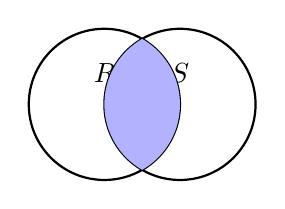
\begin{tikzpicture}[thick, scale=0.6]
          % Draw circles with 1.6 times radius
          \draw (0,0) circle(1.6cm) node[above=0.15cm] {$R$};
          \draw (1.6,0) circle(1.6cm) node[above=0.15cm] {$S$};
          
          % Intersection
          \begin{scope}
            \clip (0,0) circle(1.6cm);
            \fill[blue!30] (1.6,0) circle(1.6cm);
          \end{scope}
        \end{tikzpicture}
        \caption{Inner Join}
        \label{fig:inner-join}
      \end{subfigure}
      \hfill
      \begin{subfigure}[b]{0.24\textwidth}
        \centering
        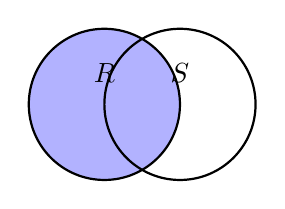
\begin{tikzpicture}[thick, scale=0.6]
          % Fill left circle
          \fill[blue!30] (0,0) circle(1.6cm);
          
          % Draw circles with 1.6 times radius
          \draw (0,0) circle(1.6cm) node[above=0.15cm] {$R$};
          \draw (1.6,0) circle(1.6cm) node[above=0.15cm] {$S$};
        \end{tikzpicture}
        \caption{Left Join}
        \label{fig:left-join}
      \end{subfigure}
      \hfill
      \begin{subfigure}[b]{0.24\textwidth}
        \centering
        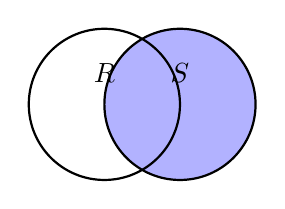
\begin{tikzpicture}[thick, scale=0.6]
          % Fill right circle
          \fill[blue!30] (1.6,0) circle(1.6cm);
          
          % Draw circles with 1.6 times radius
          \draw (0,0) circle(1.6cm) node[above=0.15cm] {$R$};
          \draw (1.6,0) circle(1.6cm) node[above=0.15cm] {$S$};
        \end{tikzpicture}
        \caption{Right Join}
        \label{fig:right-join}
      \end{subfigure}
      \hfill
      \begin{subfigure}[b]{0.24\textwidth}
        \centering
        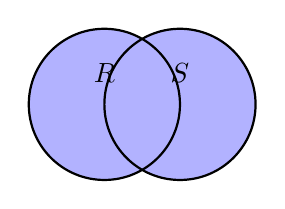
\begin{tikzpicture}[thick, scale=0.6]
          % Fill both circles
          \fill[blue!30] (0,0) circle(1.6cm);
          \fill[blue!30] (1.6,0) circle(1.6cm);
          
          % Draw circles with 1.6 times radius
          \draw (0,0) circle(1.6cm) node[above=0.15cm] {$R$};
          \draw (1.6,0) circle(1.6cm) node[above=0.15cm] {$S$};
        \end{tikzpicture}
        \caption{Full Outer Join}
        \label{fig:full-outer-join}
      \end{subfigure}
      \caption{Database join operations represented using Venn diagrams.}
      \label{fig:join-diagrams}
    \end{figure}

    \begin{example}[Outer Join]
      Consider the following relations. 

      \begin{center}
        \begin{minipage}{0.5\textwidth}
          \centering
          \begin{tabular}{|l|l|l|}
          \hline
          Name & EmpId & DeptName \\
          \hline
          Harry & 3415 & Finance \\
          Sally & 2241 & Sales \\
          George & 3401 & Finance \\
          Harriet & 2202 & Sales \\
          Tim & 1123 & Executive \\
          \hline
          \end{tabular}
        \end{minipage}%
        \begin{minipage}{0.5\textwidth}
          \centering
          \begin{tabular}{|l|l|}
          \hline
          DeptName & Manager \\
          \hline
          Sales & Harriet \\
          Production & Charles \\
          \hline
          \end{tabular}
        \end{minipage}
      \end{center}

      We demonstrate the join operations. 
      \begin{enumerate}
        \item Left outer join. 
        \begin{center}
          \begin{tabular}{|l|l|l|l|}
          \hline
          Name & EmpId & DeptName & Manager \\
          \hline
          Harry & 3415 & Finance & $\omega$ \\
          Sally & 2241 & Sales & Harriet \\
          George & 3401 & Finance & $\omega$ \\
          Harriet & 2202 & Sales & Harriet \\
          Tim & 1123 & Executive & $\omega$ \\
          \hline
          \end{tabular}
        \end{center}

        \item Right outer join. 

        \begin{center}
          \begin{tabular}{|l|l|l|l|}
          \hline
          Name & EmpId & DeptName & Manager \\
          \hline
          Sally & 2241 & Sales & Harriet \\
          Harriet & 2202 & Sales & Harriet \\
          $\omega$ & $\omega$ & Production & Charles \\
          \hline
          \end{tabular}
        \end{center}

        \item Full outer join. 
        \begin{center}
          \begin{tabular}{|l|l|l|l|}
          \hline
          Name & EmpId & DeptName & Manager \\
          \hline
          Harry & 3415 & Finance & $\omega$ \\
          Sally & 2241 & Sales & Harriet \\
          George & 3401 & Finance & $\omega$ \\
          Harriet & 2202 & Sales & Harriet \\
          Tim & 1123 & Executive & $\omega$ \\
          $\omega$ & $\omega$ & Production & Charles \\
          \hline
          \end{tabular}
        \end{center}
      \end{enumerate}
    \end{example}

  \subsubsection{Renaming}

    \begin{definition}[Renaming]
      Given a relation $R$, 
      \begin{enumerate}
        \item $\rho_S (R)$ means that you are chaning the relation name to $S$. 
        \item $\rho_{(A_1, \ldots, A_n)} (R)$ renames the attribute names to $(A_1, \ldots, A_n)$. 
        \item $\rho_{S(A_1, \ldots, A_n)} (R)$ renames the relation name to $S$ and the attribute names to $(A_1, \ldots, A_n)$. 
      \end{enumerate}
      It does not really adding any processing power. It is only used for convenience. 
    \end{definition}

  \subsubsection{Monotonicity}
    
    \begin{definition}[Monotone Operators]
      An operator $O(R)$ is monotone with respect to input $R$ if increasing the size (number of rows/tuples) of $R$ does not decrease the output relation $O$.  
      \begin{equation}
        R \subset R^\prime \implies O(R) \subset O(R^\prime)
      \end{equation}
    \end{definition}

    \begin{example}[Monotone Operators]
      Let's go through to see if each operator is monotone. 
      \begin{enumerate}
        \item Selection is monotone. 
        \item Projection is monotone. 
        \item Cross Product is monotone. 
        \item Join is monotone. 
        \item All joins are monotone w.r.t. all parameters. 
        \item Union is monotone. 
        \item Intersection is monotone. 
        \item Difference $R - S$ is monotone w.r.t. $R$ but not monotone w.r.t. $S$.
      \end{enumerate}
    \end{example}

    \begin{example}[Getting maximum of an attribute]
      Given a schema $R(a, b, c)$, how do we find the maximum of $a$? This is hard to come up in the first time since we are not allowed to compare across lines. However, we can do the following: 
      \begin{enumerate}
        \item Take the cross product of $R_1 (a_1, b_1, c_1) \times R_2 (a_2, b_2, c_2)$. 
        \item Select all tuples that are not maxes by selecting all rows where $a_1 < a_2$. The resulting rows will contain only those that are not maximums. 
      \end{enumerate}
      Therefore, we do the following 
      \begin{equation}
        \max_a (R) = [\pi_a (R) \times \pi_a (R)] - \sigma_{a_1 < a_2} [\pi_{a \mapsto a_1} (R) \times \pi_{a \mapsto a_2} (R)]
      \end{equation}
      The minimum can be solved analogously. 
    \end{example}

    Notice that the $\max_{att}$ operator is \textit{not} monotone, since the old answer is overwritten. 
    \begin{equation}
      \{\mathrm{old max}\} \not\subset \{\mathrm{new max}\}
    \end{equation}
    Generally, whenever we want to construct a non-monotone operator, we want to use the set difference since the composition of monotones is monotone. 

    You should determine when to project, before or after the difference. 

\subsection{Constraints} 

  Like mathematical structures, relational databases would not be very useful if they didn't have any structure on them. Our final database property after structure and operations are \textit{constraints}, which can also be written in relational algebra. Through it may not seem obvious, all constraints can be written with what we call \textit{set constraints}. 

  \begin{definition}[Set Constraints]
    There are two ways in which we can use relational algebra to express constraints. If $R$ and $S$ are relations, then 
    \begin{enumerate}
      \item $R = \emptyset$ constrains $R$ to be empty.
      \item $R \subset S$ constrains $R$ to be a subset of $S$.\footnote{Note that this is technically unnecessary, since we can write $R - S = \emptyset$. We can also write $R = \emptyset \iff R \subset \emptyset$.}
    \end{enumerate}
  \end{definition} 

  There are three main constraints we will look at: 
  \begin{enumerate}
    \item domain constraints 
    \item key constraints 
    \item referential integrity
  \end{enumerate}

  \subsubsection{Domain Constraints}

    There is not much to say here. We have already looked at this constraint when defining the type $T$ of an attribute $A$. That is, an instance of an attribute $A$ must be of type $T$: $a \in T$. 

    \begin{definition}[Domain Constraints]
      We can also constrain the domain of a certain attribute $r$ of relation $R$. Let $C(r)$ be the constraint. Then, 
      \begin{equation}
        \sigma_{\text{not } C(r)} (R) = \emptyset
      \end{equation}
    \end{definition}

  \subsubsection{Key Constraints}

    \begin{definition}[Key]
      A set of attributes $\mathcal{K} \subset \mathbf{A}$ form a \textbf{key} for a relation 
      \begin{enumerate}
        \item if we do not allow two tuples in any relation instance to have the same values in \textit{all} attributes of the key (i.e. in general). 
        \item no proper subset of $\mathcal{K}$ can also be a key for \textit{any} relation instance, that is, $\mathcal{K}$ is \textit{minimal}.\footnote{By minimal we do not mean that the number of attributes in $K$ is minimal. It is minimal in the sense that no proper subset of $\mathcal{K}$ can be a key.}
      \end{enumerate}
      A relation may have multiple keys, but we typically pick one as the \textbf{primary key} and underline all its attributes in the schema, e.g. \texttt{Address(\underline{street}, city, state, \underline{zip})}. 
    \end{definition}

    While we can make a key with a set of attributes, many databases use artificial keys such as unique ID numbers for safety. 

    \begin{example}[Keys of User Relation]
      Given the schema \texttt{User(uid, name, age)}, 
      \begin{enumerate}
        \item \texttt{uid} is a key of \texttt{User} 
        \item \texttt{age} is not a key (not an identifier) even if the relation at the current moment all have different ages. 
        \item \{\texttt{uid, name}\} is not a key (not minimal)
      \end{enumerate}
    \end{example}

    \begin{definition}[Key Constraints]
      If we have the key $\mathcal{K} = (k_1, \ldots, k_m) \subset \mathbf{A}$ of a relation $R$, we can express this constraint as such. We rename $R$ to copies $R_1, R_2$, denote $\mathcal{K}^\prime = \mathbf{A} - \mathcal{K}$, and write 
      \begin{equation}
        \sigma_{R_1.\mathcal{K} = R_2.\mathcal{K} \text{ and } R_1.\mathcal{K}^\prime \neq R_2.\mathcal{K}^\prime} (R_1 \times R_2) = \emptyset
      \end{equation}
      That is, if we found a $r_1 \in R_1, r_2 \in R_2$ that matched in the key attributes, then it must be the case that $r_1 = r_2$. But if they are equal in the rest of the attributes, they will be projected out. 
    \end{definition}

  \subsubsection{Referential Integrity}

    \begin{definition}[Referential Integrity Constraints]
      One way that we can use this is through \textit{referential integrity} constraints, which asserts that a value appearing as an attribute $r$ in relation $R$ also should appear in a value of an attribute $s$ in relation $S$. That is, 
      \begin{equation}
        \pi_r (R) \subset \pi_s (S)
      \end{equation}
    \end{definition}

\subsection{Functional Dependencies} 

    A generalization of keys is functional dependencies. Since it can be viewed as another form of key constraint, it is included here, but it is also a method of describing relationships within data, which will be useful in effective designing of databases.  

    \begin{definition}[Functional Dependency]
      Given a relation $R$ with attributes $\mathbf{A}$, let $\mathbf{a} = (a_1, \ldots, a_n), \mathbf{b} = (b_1, \ldots, b_m) \subset \mathbf{A}$. Then, the constraint 
      \begin{equation}
        \mathbf{a} \mapsto \mathbf{b}
      \end{equation}
      also called ``$\mathbf{a}$ \textbf{functionally determines} $\mathbf{b}$,'' means that if two tuples agree on $\mathbf{a}$, then they must agree on $\mathbf{b}$. We say that $R$ satisfies a FD $f: \mathbf{a} \mapsto \mathbf{b}$ or a set of FDs $F = \{f\}$ if this constraint is satisfied. 
    \end{definition}

    From this, we can see that the term ``functional'' comes from a literal function being defined on the input $\mathbf{a}$. 

    \begin{lemma}[FDs as Key Constraints]
      Note that the functional dependency $\mathbf{a} \mapsto \mathbf{b}$ also implies the key constraint 
      \begin{equation}
        \sigma_{R_1.\mathbf{a} = R_2.\mathbf{a} \text{ and } R_1.\mathbf{b} \neq R_2.\mathbf{b}^\prime} (R_1 \times R_2) = \emptyset
      \end{equation}
    \end{lemma}

    \begin{definition}[Superkey]
      A set of attributes $\mathbf{k}$ of a relation $R$ is called a \textbf{superkey} if 
      \begin{equation}
        \mathbf{k} \mapsto \mathbf{r} - \mathbf{k}
      \end{equation}
      If no $\mathbf{k}^\prime \subset \mathbf{k}$ functionally determines $\mathbf{r}$, then it is a key. 
    \end{definition}
    
    \begin{example}[Clarification of Minimal Meaning]
      Given a relation $R(A, B, C, D, E, F)$ with functional dependencies 
      \begin{equation}
        AEF \mapsto C, BF \mapsto C, EF \mapsto D, ACDE \mapsto F
      \end{equation}
      We can see that every attribute not on the right hand side ($C, D, F$) must be a key. If we do a bit of testing out, we can see that 
      \begin{enumerate}
        \item $ABEF$ is a key. 
        \item $ABCDE$ is also a key since even though it has 5 attributes, it is minimal in the sense that no proper subset functionally determines every other attribute.   
      \end{enumerate}
    \end{example}

  \subsubsection{Structure on Spaces of Functional Dependencies}

    To introduce additional structure, we will introduce two spaces. 
    \begin{enumerate}
      \item Given a relation $R$, let us consider the set of all FDs $F = F(R)$ on $R$. This is clearly a large set, which increases exponentially w.r.t. the number of attributes in $R$. 
      \item Let us denote the set of all relations $R$ satisfying $F$ as $R_F$, which is an infinite set. 
    \end{enumerate}

    \begin{theorem}[Armstrong Axioms]
      Let's prove a few properties of FDs, which have nice structure. 
      \begin{enumerate}
        \item \textit{Splitting and Combining}. The two sets of FDs are equal. 
          \begin{equation}
            \{\mathbf{a} \mapsto \mathbf{b}\} \iff \{ \mathbf{a} \mapsto b_i \mid i = 1, \ldots, m\}
          \end{equation}

        \item \textit{Trivial FDs}. Clearly elements of $\mathbf{a}$ uniquely determines its own attributes. 
          \begin{equation}
            \mathbf{a} \mapsto \mathbf{b} \implies \mathbf{a} \mapsto \mathbf{b} - \mathbf{a}
          \end{equation}
          or can also be written as 
          \begin{equation}
            \mathbf{b} \subset \mathbf{a} \implies \mathbf{a} \mapsto \mathbf{b}
          \end{equation}

        \item \textit{Augmentation}. 
          \begin{equation}
            \mathbf{a} \mapsto \mathbf{b} \implies \mathbf{a}, \mathbf{c} \mapsto \mathbf{b}, \mathbf{c}
          \end{equation}

        \item \textit{Transitivity}. If $\mathbf{a} \mapsto \mathbf{b}, \mathbf{b} \mapsto \mathbf{c}$, then 
          \begin{equation}
            \mathbf{a} \mapsto \mathbf{c}
          \end{equation}
      \end{enumerate}
    \end{theorem}
    \begin{proof}
      Trivial. 
    \end{proof}

    It is also possible to put a partial order on $F$. 

    \begin{definition}[Partial Order]
      Given two FDs $f$ and $g$, consider the set of all relations $R$ satisfying $f$ and $g$, denoted as $R_f$ and $R_g$. 
      \begin{enumerate}
        \item Then $f \implies g$ iff $R_f \subset R_g$. 
        \item $f \iff g$ iff $R_f = R_g$. 
      \end{enumerate}
    \end{definition}

    Moreover, we can use this structure on $F$ to induce structure on the set of attributes $\mathbf{r}$. 

    \begin{definition}[Closure of Attributes]
      The \textbf{closure} of $\mathbf{r}$ under a set of FDs $F$ is the set of attributes $\mathbf{b}$ s.t. 
      \begin{equation}
        R_F = R_\mathbf{b}
      \end{equation}
      We denote this as $\mathbf{b} = \mathbf{r}^+$. To actually compute the closure, we take a greedy approach by starting with $\mathbf{r}$ and incrementally adding attributes satisfying $F$ until we cannot add any more. 
    \end{definition}

    \begin{theorem}[Implication of Functional Dependencies]
      If we want to know where one FD $f: \mathbf{a} \mapsto \mathbf{b}$ follows from a set $F$ of functional dependencies, 
      \begin{enumerate}
        \item We compute the closure $\mathbf{a}^+$ w.r.t. $F$. 
        \item If $\mathbf{b} \subset \mathbf{a}^+$, then $f$ follows from $F$. 
      \end{enumerate}
      Alternatively, we can also use the \textit{Armstrong axioms} above to derive all implications. 
    \end{theorem}
  
  \subsubsection{Projections of Functional Dependencies} 

    If we have a relation $R$ with a set of FDs $F$, and we project $R^\prime = \pi_{\mathbf{r}^\prime} (R)$, then the set of FDs $F^\prime$ that hold for $R^\prime$ consists of 
    \begin{enumerate}
      \item The FDs that follow from $F$, and 
      \item involve only attributes of $R$. 
    \end{enumerate} 

    Calculating the FDs that hold is not trivial, and the calculations of the FDs for $R^\prime$ is exponential in the number of attributes of $R^\prime$. 

    \begin{theorem}[Calculating Projections of Functional Dependencies]
      Given a relation $R$ and its set of functional dependencies $F$, let $R^\prime = \pi(R)$ be a projection. 
      \begin{enumerate}
        \item Let $G$ be the set of FDs that we construct that hold for $R^\prime$. Initially it is empty. 
        \item For each set of attributes $\mathbf{r}$ that is a subset of the attributes of $R_1$, compute $\mathbf{r}^+$. This computation is performed w.r.t. the set of FDs in $S$, and may involve attributes in the schema of $R$ but not in $R^\prime$. Add to $G$ all nontrivial FDs $\mathbf{r} \rightarrow A$ such that $A$ is both in $\mathbf{r}^+$ and an attribute in $R^\prime$. 
      \end{enumerate}
      This gives our projection, but it may not be minimal. To make it minimal, repeat the two steps, independently. 
      \begin{enumerate}
        \item If there is an FD $g$ in $G$ that follows from the other FDs in $G$, remove $g$. 
        \item Let $g = \mathbf{a} \mapsto \mathbf{b} $ be an FD in $G$, with at least 2 attributes in $\mathbf{a}$, and let $\mathbf{a}^\prime$ be $\mathbf{a}$ with one of its attributes removed. If $g^\prime = \mathbf{a}^\prime \mapsto \mathbf{b}$ follows from the FDs in $G$ (including $g$), then replace $g$ with $g^\prime$. 
      \end{enumerate}
      Once neither step can be done, we have a minimal set. 
    \end{theorem}

    \begin{example}[Computing FDs for Projections]
      Suppose $R(A,B,C,D)$ has FD's $A \rightarrow B$, $B \rightarrow C$, and $C \rightarrow D$. Suppose also that we wish to project out the attribute $B$, leaving a relation $R_1(A,C,D)$. In principle, to find the FD's for $R_1$, we need to take the closure of all eight subsets of $\{A, C, D\}$, using the full set of FD's, including those involving $B$. However, there are some obvious simplifications we can make.

      \begin{itemize}
        \item Closing the empty set and the set of all attributes cannot yield a nontrivial FD.
        \item If we already know that the closure of some set $X$ is all attributes, then we cannot discover any new FD's by closing supersets of $X$.
      \end{itemize}

      Thus, we may start with the closures of the singleton sets, and then move on to the doubleton sets if necessary. For each closure of a set $X$, we add the FD $X \rightarrow E$ for each attribute $E$ that is in $X^+$ and in the schema of $R_1$, but not in $X$.

      First, $\{A\}^+ = \{A,B,C,D\}$. Thus, $A \rightarrow C$ and $A \rightarrow D$ hold in $R_1$. Note that $A \rightarrow B$ is true in $R$, but makes no sense in $R_1$, because $B$ is not an attribute of $R_1$.

      Next, we consider $\{C\}^+ = \{C,D\}$, from which we get the additional FD $C \rightarrow D$ for $R_1$. Since $\{D\}^+ = \{D\}$, we can add no more FD's, and are done with the singletons.

      Since $\{A\}^+$ includes all attributes of $R_1$, there is no point in considering any superset of $\{A\}$. The reason is that whatever FD we could discover, for instance $AC \rightarrow D$, follows from an FD with only $A$ on the left side: $A \rightarrow D$ in this case. Thus, the only doubleton whose closure we need to take is $\{C, D\}^+ = \{C,D\}$. This observation allows us to add nothing. We are done with the closures, and the FD's we have discovered are $A \rightarrow C$, $A \rightarrow D$, and $C \rightarrow D$.

      If we wish, we can observe that $A \rightarrow D$ follows from the other two by transitivity. Therefore a simpler, equivalent set of FD's for $R_1$ is $A \rightarrow C$ and $C \rightarrow D$. This set is, in fact, a minimal basis for the FD's of $R_1$. 
    \end{example}

